%%
%% This is file `mcmthesis-demo.tex',
%% generated with the docstrip utility.
%%
%% The original source files were:
%%
%% mcmthesis.dtx  (with options: `demo')
%% !Mode:: "TeX:UTF-8"
%% -----------------------------------
%%
%% This is a generated file.
%%
%% Copyright (C)
%%     2010 -- 2015 by latexstudio
%%     2014 -- 2016 by Liam Huang
%%
%% This work may be distributed and/or modified under the
%% conditions of the LaTeX Project Public License, either version 1.3
%% of this license or (at your option) any later version.
%% The latest version of this license is in
%%   http://www.latex-project.org/lppl.txt
%% and version 1.3 or later is part of all distributions of LaTeX
%% version 2005/12/01 or later.
%%
%% This work has the LPPL maintenance status `maintained'.
%%
%% The Current Maintainer of this work is Liam Huang.
%%
\documentclass{mcmthesis}
\mcmsetup{CTeX = true,   % 使用 CTeX 套装时,设置为 true
        tcn = 0000, problem = B,
        sheet = true, titleinsheet = true, keywordsinsheet = true,
        titlepage = false, abstract = true}
\usepackage{palatino}
\usepackage{lipsum}
\title{The \LaTeX{} Template for MCM Version \MCMversion}
\author{\small \href{http://www.latexstudio.net/}
  {
\includegraphics[width=7cm]{mcmthesis-logo}}}
\date{\today}
\begin{document}
\begin{abstract}
\lipsum[1]%写summary的地方
\begin{keywords}
keyword1; keyword2
\end{keywords}
\end{abstract}
\maketitle
\tableofcontents
\newpage

\section{Introduction}
\subsection{Background}

Lewis Mumford, a famous sociologist and literary critic,
once said in a metaphorical manner, ``Adding highway lanes
to deal with traffic congestion is like loosening your
belt to cure obesity.`` Fortunately, he did not experience
the worse congestion around today`s highway toll plaza.

Currently, with roaring number of vehicles, rising
construction costs and constrained available areas,
traffic jam becomes more and more serious but future
toll-plaza construction opportunities are limited to
improve this situation markedly. Figure 1 shows the
congestion in the toll plaza near Tappan Zee Bridge.

\begin{figure}[h]
\small
\centering
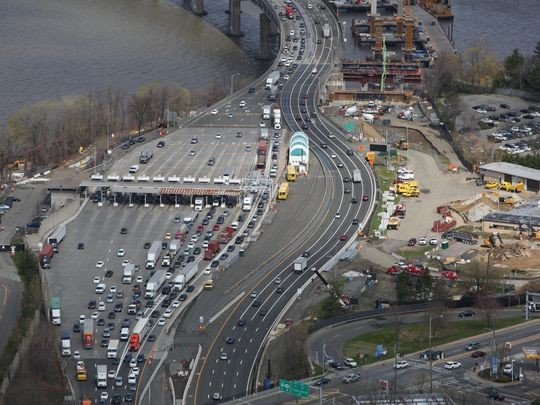
\includegraphics[width=10cm]{figure1}
\caption{Toll plaza congestion}\label{fig1}
\end{figure}

Subject to the constraints referred above, neither
increasing highway lanes nor building more tollbooths
seems practical enough to relieve traffic jam around a
toll plaza nowadays, particularly for some heavily-traveled
 roads such as the Garden State Parkway, New Jersey.
 Therefore, looking for some innovative design improvements
  on the geometric parameters of the extent toll plaza
  is an effective solution.


\subsection{Restatement of the Problem}
In this paper, we are required to explore if there is a
better-than-ever toll plaza model with specific shape,
size, and merging pattern. In this model, the prerequisite
is that vehicles fan in from B tollbooth egress lanes down
to L (B\textgreater L) lanes of traffic (i.e., the number of both
tollbooths and the lanes after merging are fixed). We aim
to construct a model that can optimize the arrangement
according to the following conditions.

\begin{itemize}
\item Enhance the capability of the accident prevention(A).
\item Maximize the throughput(T).
\item Minimize the cost of the land and road
construction(C).
\end{itemize}

Through our analysis, we determine if there are better
solutions than any toll plaza in common use. Afterwards,
the performance of our solution in light and heavy traffic
and other various situations along with corresponding
sensitivity analysis is discussed.


\section{Notations}

\section{Model 1: The Traffic Throughput Model}
\subsection{Overview}
We manage to design two sub-models to analyze and
calculate the maximum throughput in three parts
(i.e., the approach zone, the tollbooth area, and
the departure zone) of the toll plaza. And we define
this throughput as $Q_{1max}$ and $Q_{2max}$ together,
$Q_{3max}$ respectively. $Q_{1max}$ and $Q_{2max}$ can
be viewed as the properties of upstream, while $Q_{3max}$
 is for downstream. We assume corresponding ideal
 conditions to apply on respective calculation, and
 related assumptions will be displayed in the following
 chapters. In view of the Buckets Effect, the overall
 the maximal traffic flow $Q_{max}$ is determined by
 the minimum among the three values, that is:
\[{Q_{\max }} = \min \left\{ {{Q_{1\max }},{Q_{2\max }},{Q_{3\max }}} \right\}\]
Figure 2 illustrates the schematic diagram of the whole.

\begin{figure}[h]
\small
\centering
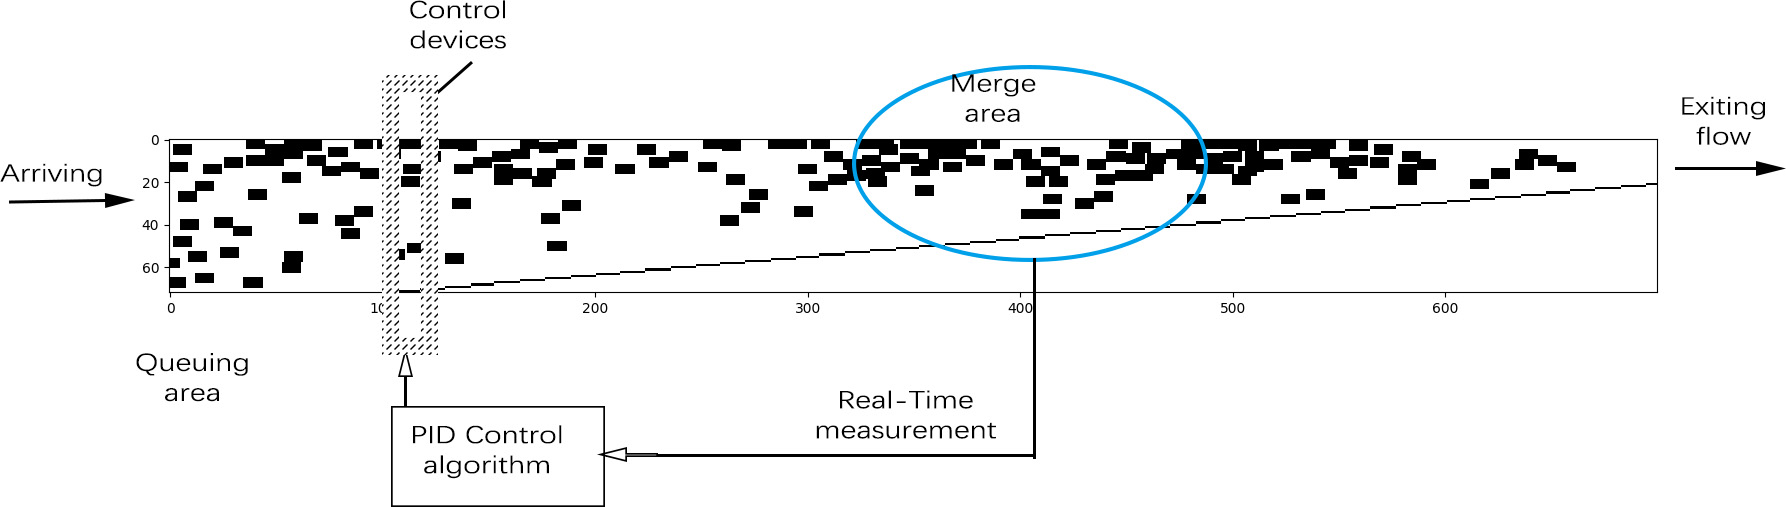
\includegraphics[width=13cm]{figure2}
\caption{the schematic diagram of the whole}\label{fig2}
\end{figure}
%此处的figure2被放到了下一页

We need to further explain that $Q_{i}$ is the number of
vehicles passing through the cross-section $S_{i}$ within
a certain time, where i = 1,2,3. Because our main
subject is $Q_{3}$, which relates directly to subsequent
analysis of the shape, size and merging pattern of
the departure zone, sub-model 2(the downstream flow
model) is more complicated than the former. Relatively
simple as sub-model 1(the upstream flow model) is, it
still acts as an indispensable tool to help define
crucial parameters in sub-mode 2.

The first model is determined to simulate the maximum
flow $Q_{1}$ in the approach, which is also interpreted as
the vehicle flow under the ``optimal occupancy`` of the
approach zone. The ``optimal occupancy`` is set to describe
a critical ratio of real-time cars amount to the maximum
capacity in the approach zone. If the real-time radio is
 higher than the critical value, the upstream tends to
 congest gradually next time. While lower, the situation
 is defined as a smooth or normal one. In other words,


\[
  p_{j}=\begin{cases} 0,&\text{if $j$ is odd}\\
  r!\,(-1)^{j/2},&\text{if $j$ is even}
  \end{cases}
\]

\lipsum[10]

\[
  \arcsin \theta  =
  \mathop{{\int\!\!\!\!\!\int\!\!\!\!\!\int}\mkern-31.2mu
  \bigodot}\limits_\varphi
  {\mathop {\lim }\limits_{x \to \infty } \frac{{n!}}{{r!\left( {n - r}
  \right)!}}} \eqno (1)
\]

\section{Calculating and Simplifying the Model  }
\lipsum[11]

\section{The Model Results}
\lipsum[6]

\section{Validating the Model}
\lipsum[9]

\section{Conclusions}
\lipsum[6]

\section{A Summary}
\lipsum[6]

\section{Evaluate of the Mode}

\section{Strengths and weaknesses}
\lipsum[12]

\subsection{Strengths}
\begin{itemize}
\item \textbf{Applies widely}\\
This  system can be used for many types of airplanes, and it also
solves the interference during  the procedure of the boarding
airplane,as described above we can get to the  optimization
boarding time.We also know that all the service is automate.
\item \textbf{Improve the quality of the airport service}\\
Balancing the cost of the cost and the benefit, it will bring in
more convenient  for airport and passengers.It also saves many
human resources for the airline. \item \textbf{}
\end{itemize}

\begin{thebibliography}{99}
\bibitem{1} D. E. KNUTH   The \TeX{}book  the American
Mathematical Society and Addison-Wesley
Publishing Company , 1984-1986.
\bibitem{2}Lamport, Leslie,  \LaTeX{}: `` A Document Preparation System '',
Addison-Wesley Publishing Company, 1986.
\bibitem{3}\url{http://www.latexstudio.net/}
\bibitem{4}\url{http://www.chinatex.org/}
\end{thebibliography}

\begin{appendices}

\section{First appendix}

\lipsum[13]

Here are simulation programmes we used in our model as follow.\\

\textbf{\textcolor[rgb]{0.98,0.00,0.00}{Input matlab source:}}
\lstinputlisting[language=Matlab]{./code/mcmthesis-matlab1.m}

\section{Second appendix}

some more text \textcolor[rgb]{0.98,0.00,0.00}{\textbf{Input C++ source:}}
\lstinputlisting[language=C++]{./code/mcmthesis-sudoku.cpp}

\end{appendices}
\end{document}

%%
%% This work consists of these files mcmthesis.dtx,
%%                                   figures/ and
%%                                   code/,
%% and the derived files             mcmthesis.cls,
%%                                   mcmthesis-demo.tex,
%%                                   README,
%%                                   LICENSE,
%%                                   mcmthesis.pdf and
%%                                   mcmthesis-demo.pdf.
%%
%% End of file `mcmthesis-demo.tex'.
